\documentclass[12pt,a4paper]{article}
\usepackage{amsmath}
\usepackage{amsfonts}
\usepackage{amssymb}
\usepackage{graphicx}
\usepackage{secdot}
\usepackage{multirow}
\usepackage[left=2cm,right=2cm,top=2cm,bottom=2cm]{geometry}

\title{{Experiment - 7\\ \textbf{Flow over a symmetrical airfoil NACA0015}}}
\author{Arka Pramanick, AE21B007\\ Department of Aerospace Engineering\\ IIT Madras\\[3ex] Instructor:\\ \large Professor Dr. R. Sriram}

\date{03 April, 2023}


\begin{document}
\maketitle

\hline

\section{Aim :}
\begin{itemize}
    \item To find $C_p$ on NACA0015 at various angle of attack.
    \item To estimate $C_l$ and $C_d$ for various angle of attack.
\end{itemize}


\section{Apparatus :}
Required apparatus for performing this experiment are:
\begin{itemize}
    \item Manometer
    \item C15-10 Armfield tunnel
    \item Pitot-static Probe
    \item Fan
    \item NACA0015 Symmetric airfoil
\end{itemize}



\newpage
\section{Theory :}

NACA0015 is a relatively thin and symmetric airfoil,so we can apply 'Thin Airfoil Theory' to determine theoretical values of Lift,Drag and moment Coefficients.
The angle of attack is the angle between the chord line of an airfoil and an the oncoming air. A symmetrical airfoil generates zero lift at zero angle of attack.On increasing angle of attack ,the air deflects through larger angle and vertical component of airstream velocity increases which generates more Lift.
\underline{\textbf{Coefficients of Lift($C_l)$}} :\\
Coefficients of Lift is the dimentionless quantity which measure the lift generated by a lifting body to the fluid density around the body.\\
Theoretically, $$C_l = 2 \pi\alpha$$ \\
$C_l$ can be calculated from pressure tap data as :
$$ C_l = \int_{TE}^{LE} \{(C_p)_{l} - (C_p)_{u}\} \,d(\frac{y}{c}) $$





\underline{\textbf{Drag}} : Drag is the force which opposes the motion of an object.
Drag is calculated by : \\
$$D = \int_{-\infty}^{\infty} \rho v (V_{\infty}-v)\,dy $$
\underline{\textbf{Coefficients of Drag }} :
Drag coefficients caused due to skin friction and Drag. Drag coefficients is calculated by :
$$ C_d = \frac{D}{(\rho V_{\infty}^2 d)/2} $$ \\
$C_d$ can be calculated from pressure tap data too as following :
$$ C_d = \int_{TE}^{LE} \{(C_p)_{l} - (C_p)_{u}\} \,d(\frac{x}{c}) $$



\underline{\textbf{Reynolds Number :}}
The Reynolds number is the ratio of inertial forces to viscous forces within a fluid which is subjected to relative internal moment due to variation of velocities.
$$  R_e = \frac{\rho V_{\infty d}}{\mu} $$
For a thin airfoil Reynolds No can be calculated as :
$$ R_e = \frac{Vc}{\nu} $$
where, V = Flight speed,\\
c = Chord length ,\\
$\nu$ = Kinematics of the fluid in which the airfoil operates, for the atmosphere  at sea level $\nu =  1.46\times 10^{-5} \frac{m^{2}}{s} $\\







\section{Procedure :}
\begin{enumerate}
    \item In wind tunnel test section is set.
    \item Pitot-static probe is connected to manometer.
    \item Fan speed is fixed.
    \item Angle of attack is fixed
    \item Required readings are taken.
\end{enumerate}






\section{Observation :}
Air velocity = 15.2 m/s \\
Angle of attack = $4^{\circ}$

\subsection{Pressure distribution and $C_p$ for upper surface of airfoil }
\begin{table}[ht]
\centering
\caption{\textbf{Pressure distribution and $C_p$ for upper surface of airfoil }}
\vspace{2mm}

\begin{tabular}{|p{10mm}|p{20mm}|p{20mm}|p{20mm}|p{20mm}|} 
 \hline
Port No. & Tapping point location from starting point(in mm) & Stagnation Pressure(in mm of water) & (P- $P_{\infty}$)(in Pa) &  $(C_p)_u$ \\  
 \hline
$P_1$ & 0 & -4.4  & 43.164 & 0.289 \\ 
 \hline
$P_2$ & 3 & -31.1 & 305.091 & 2.043 \\
 \hline
$P_3$ & 5 & -28.5 & 279.585 & 1.872 \\
 \hline
 $P_4$ & 7 & -30.3 & 297.243 & 1.990 \\
 \hline
$P_5$ & 9 & -27.7 & 271.737 & 1.819\\
 \hline
$P_6$ & 22 & -25.2 & 247.212 & 1.655\\ 
 \hline
$P_7$ & 29 & -24.2 & 237.402 & 1.589 \\ 
 \hline
$P_8$ & 36 & -21.6 & 211.896 & 1.419 \\
 \hline
$P_9$ & 43 & -19.0 & 186.39 & 1.248 \\
 \hline
$P_{10}$ & 50 & -17.3 & 169.713 & 1.136 \\ 
 \hline 

\end{tabular}

\end{table}

\begin{figure}[!ht]
	\begin{center}
		\framebox{
			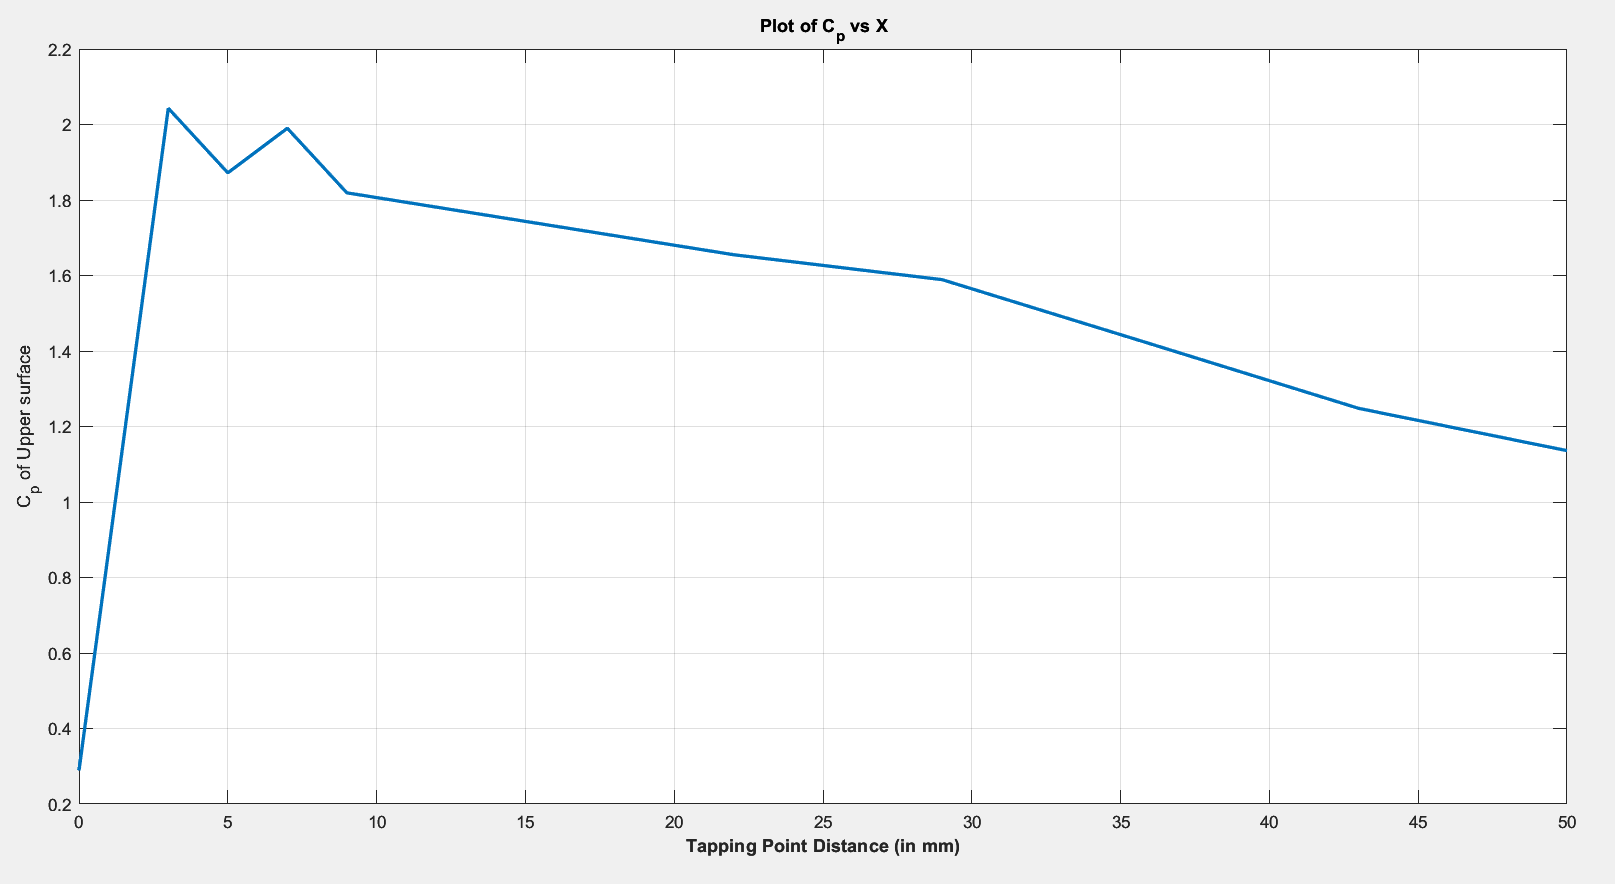
\includegraphics[scale=0.4]{cp vs x.png}
		}
	\end{center}
	\caption{Variation of $C_P$ with X distance of pitot tube}
\end{figure}




\begin{table}[ht]
\centering
\caption{\textbf{Calculation of $C_p$ of Upper surface of Airfoil}}
\vspace{2mm}

\begin{tabular}{|p{10mm}|p{20mm}|p{20mm}|p{20mm}|p{20mm}|} 
 \hline
Port No. & Tapping point location from starting point(in mm) & Stagnation Pressure(in mm of water) & (P- $P_{\infty}$)(in Pa) &  $(C_p)_l$ \\  
 \hline
$P_1$ & 0 & -6.9  & 67.689 & 0.453 \\ 
 \hline
$P_2$ & 3 & -10.5 & 103.005 & 0.690 \\
 \hline
$P_3$ & 5 & -9.6 & 94.176 & 0.630 \\
 \hline
 $P_4$ & 7 & -13.6 & 133.416 & 0.893 \\
 \hline
$P_5$ & 9 & -16.1 & 157.941 & 1.057 \\
 \hline
$P_6$ & 22 & -16.7 & 163.827 & 1.097 \\ 
 \hline
$P_7$ & 29 & -16.2 & 158.922 & 1.064 \\ 
 \hline
$P_8$ & 36 & -14.3 & 140.283 & 0.939 \\
 \hline
$P_9$ & 43 & -14.9 & 146.169 & 0.979 \\
 \hline
$P_{10}$ & 50 & -14.1 & 138.321 & 0.926 \\ 
 \hline 

\end{tabular}

\end{table}











\newpage

\begin{table}[ht]
\centering
\caption{\textbf{Determination of X and Corresponding Y}}
\vspace{2mm}

\begin{tabular}{|p{10mm}|p{20mm}|p{20mm}|p{20mm}|p{20mm}|} 
 \hline
Port No. & Tapping point location from starting point(in mm)(X) & Correspon-ding 
value of Y (in mm) & $\Delta X$ &  $\Delta Y$ \\  
 \hline
$P_1$ & 0 & 0  & 0 & 0 \\ 
 \hline
$P_2$ & 3 & 2.7908 & 3 & 2.7908 \\
 \hline
$P_3$ & 5 & 3.4465 & 2 & 0.6557 \\
 \hline
 $P_4$ & 7 & 3.9062 & 2 & 0.4597 \\
 \hline
$P_5$ & 9 & 4.2417 & 2 & 0.3355\\
 \hline
$P_6$ & 22 & 4.8504 & 13 & 0.6087\\ 
 \hline
$P_7$ & 29 & 4.5502 & 7 & -0.3002 \\ 
 \hline
$P_8$ & 36 & 4.0008 & 7 & -0.5494 \\
 \hline
$P_9$ & 43 & 3.2724 & 7 & -0.7284 \\
 \hline
$P_{10}$ & 50 & 2.4031 & 7 & -0.8693 \\ 
 \hline 

\end{tabular}

\end{table}


\begin{figure}[!ht]
	\begin{center}
		\framebox{
			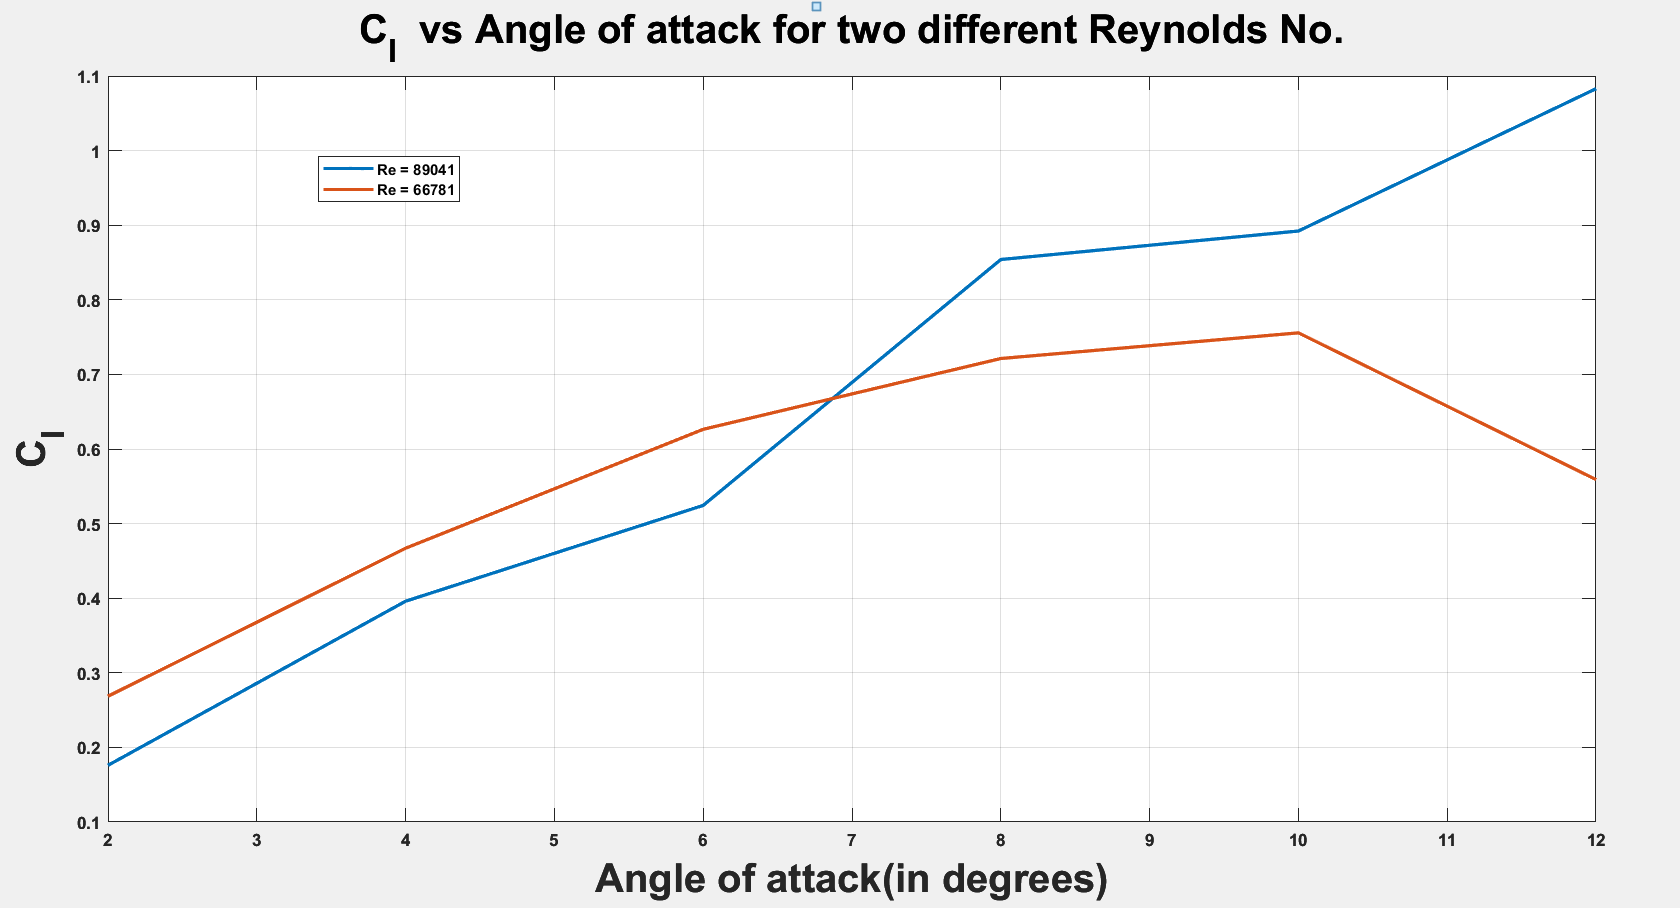
\includegraphics[scale=0.4]{cl vs alpha.png}
		}
	\end{center}
	\caption{Variation of Coefficients of Lift with Angle of attack for different Reynolds No.}
\end{figure}


\begin{figure}[!ht]
	\begin{center}
		\framebox{
			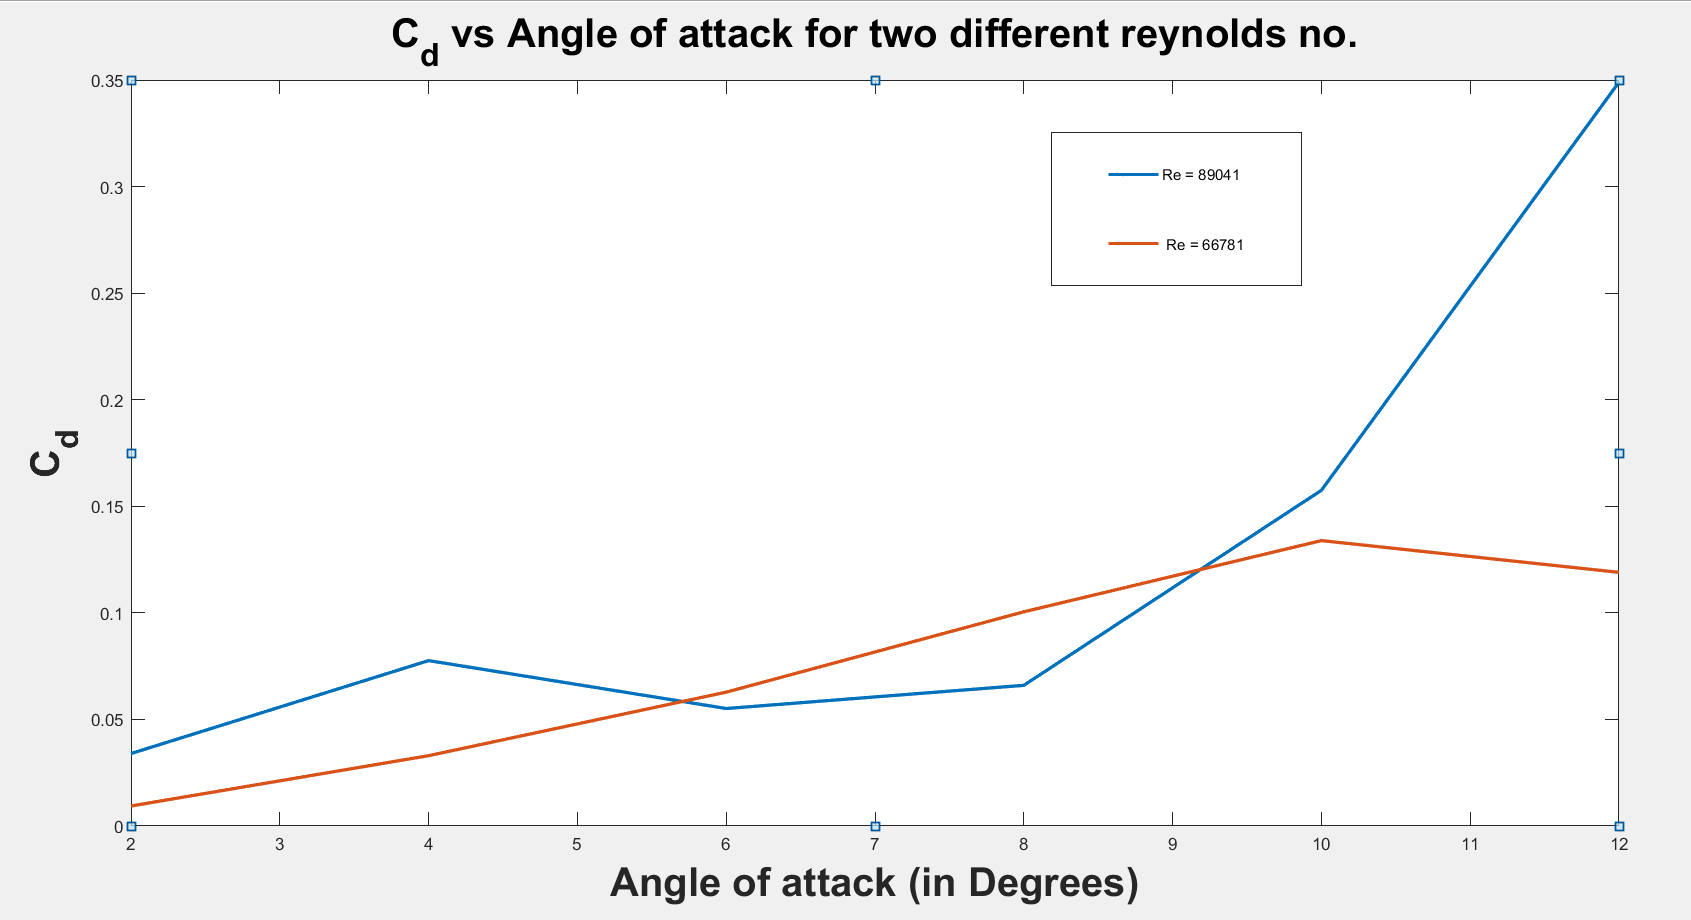
\includegraphics[scale=0.4]{cd vs alpha.png}
		}
	\end{center}
	\caption{Variation of Coefficients of Drag with Angle of attack for different Reynolds No.}
\end{figure}

\clearpage
 

\section{Calculations :}
Density of air = 1.293 $m^3$ \\
Density of Water($\rho_{w}$) = 1000 $Kg/m^3$

\subsection{Calculation of Coefficient of Lift($C_l$)}
Coefficient of Lift($C_l$) is calculated by , \\
For 10 ports,\[ C_l = \int_{TE}^{LE} \{(C_p)_{l} - (C_p)_{u}\} \,d(\frac{y}{c})  \approx  \sum_{i=1}^{9} \frac{\{((C_p)_{l} - (C_p)_{u})_{avg}\}_i (\Delta y)_i}{c}\ \]

Where, $ (((C_p)_{l} - (C_p)_{u})_{avg})_i = \frac{((C_p)_{l} - (C_p)_{u})_{i}+((C_p)_{l} - (C_p)_{u})_{i+1}}{2}$ \\
$\Delta y = y_{i+1} - y_i$ \\
c = Chord length = 65 mm\\



For port 1 \& 2, \\
\begin{align*}
    ((C_p)_{l} - (C_p)_{u})_{avg}) &=  \frac{((C_p)_{l} - (C_p)_{u})_{i}+((C_p)_{l} - (C_p)_{u})_{i+1}}{2} \\
    &=\frac{(0.453-0.289)+(0.690-2.043)}{2} \\
    \Delta y = y_{2}-y_{1} = 2.7908 mm\\
    \therefore (C_l)_1 = -0.0255
\end{align*}

In this way can get $C_d$ contribution due to each port.\\
Therefore

$$\framebox{$C_l$ = 0.0436}$$




\subsection{Calculation of Coefficient of Drag($C_d$) :}
Coefficient of Drag(D) is calculated by , \\
For 10 ports,\[ C_d = \int_{TE}^{LE} \{(C_p)_{l} - (C_p)_{u}\} \,d(\frac{x}{c})  \approx  \sum_{i=1}^{9} \frac{\{((C_p)_{l} - (C_p)_{u})_{avg}\}_i (\Delta x)_i}{c}\ \]

Where, $ (((C_p)_{l} - (C_p)_{u})_{avg})_i = \frac{((C_p)_{l} - (C_p)_{u})_{i}+((C_p)_{l} - (C_p)_{u})_{i+1}}{2}$ \\
$\Delta x = x_{i+1} - x_i$ \\
c = Chord length = 65 mm\\



For port 1 \& 2, \\
\begin{align*}
    ((C_p)_{l} - (C_p)_{u})_{avg}) &=  \frac{((C_p)_{l} - (C_p)_{u})_{i}+((C_p)_{l} - (C_p)_{u})_{i+1}}{2} \\
    &=\frac{(0.453-0.289)+(0.690-2.043)}{2} \\
    \Delta x = x_{2}-x_{1} = 3 mm\\
    \therefore (C_d)_1 = -0.027
\end{align*}

In this way can get $C_d$ contribution due to each port.\\
Therefore

$C_d$ = [0.027+0.0399+0.036+0.0286+0.13+0.057+0.054+0.04+0.026]= 0.4385

$$\framebox{ $C_d$ = 0.4385} $$






\subsection{Calculation of  Reynolds number($R_e$):}
$$ Reynolds No.(R_e) = \frac{Vc}{\nu}$$ \\


where,\\
$\nu = Kinematic Viscosity = 1.46\times 10^{-5} \frac{m^{2}}{s}$(for the atmosphere at sea level.)\\
V = Flight speed\\
c = Chord length

Reynolds No.(Re) = $\frac{Vc}{\nu}$ \\



For velocity(V) = 15.2 m/s, \\
\begin{align*}
    R_e &= \frac{Vc}{\nu} \\
    &= \frac{15.2\times65\times 10^{-3}}{1.46\times 10^{-5}}\\
    R_e &= 67671.23 
\end{align*}





\section{Sources of Error:}
\begin{itemize}
    \item Error due to instrumental defect.
    \item Error may occur in taking readings before flow becomes steady.
    \item Error due to environmental effect like temperature,pressure change.
    \item Error in measurement due to presence of zero error in parameters.
    \item Dimensional error may occurs 
\end{itemize}



\section{Conclusion :}
\begin{itemize}
    \item On increasing angle of attack more lift is generated.
    \item On increasing angle of attack Coefficient of Drag increases.  
    \item At $0^{\circ}$ Angle of attack pressure distribution line is symmetry about each other on both upper and lower surface.
    \item As angle of attack increases at leading edge flow seperation occurs and at trailing edge pressure rises suddenly.
\end{itemize}


\end{document}